\chapter{Traceability Matrix} \labchap{traceability_matrix}
A traceability matrix is an artifact within Systems Engineering that tracks the stakeholder requirements, capabilities, system requirements, and testing methodologies.
The primary purpose is to give a Lead Systems Engineer other other team member quick access to all of the driving information for the product and trace the requirement lifecycle.
Each matrix has eight columns that contain information about the requirement:

\paragraph*{ID} This is the identification number for the requirement.
Stakeholder requirements will start with the prefix: ``SR''.
Capabilities will be triple-digit numbers with 100-level being ``threshold'', 200-level being ``reach'', and 300-level being ``stretch'' capabilities.
Component-level requirements will be divided into sections and subsections in the format ``X.X.X.X'' depending on the section and depth of the requirement.
For example, the first requirement in the first section, first subsection of the component-level matrix will have the ID ``1.1.1''.

\paragraph*{Description} Each requirement and capability needs to have a brief, single sentence description that details the feature.
The description should follow the guidelines laid out by NASA \cite{SystemsEngineeringHandbook-AppendixC}.
They should be unambiguous, testable, verifiable, and consistent in both terminology and can either be functional or non-functional.
Functional requirements directly drive a feature of the product, whereas a non-functional requirement drives an aesthetic or interface choice.

\paragraph*{Weight} The requirements and capabilities should all have a weight associated with them.
These can be based on stakeholder preferences, developer capabilities, technology limitations, etc.
The weight is a number greater than 0, but less than 1 and typically only expressed to two decimal places.

\paragraph*{Priority} Derived from the weight, the priority is the relative importance of a particular requirement or capability to others.
It is calculated using Equation \ref{eq:priority}. 
A higher priority means a requirement is more important to implement on the product.
For capabilities, the priority is calculated slightly differently.
The weight of a capability is compared to all of the other weights in the same category and the one(s) beneath it.
For instance, a threshold capability's priority will only factor in the weights of other threshold capabilities.
But, a stretch capability's priority will factor in the weights of all capabilities in the design.

\begin{equation} \labeq{priority}
    P = \frac{w_c}{\sum w} \times 100
\end{equation}

\paragraph*{Owner} The person who is responsible for a requirement or capability is called the owner.
This individual is in charge of developing, implementing, verifying, testing, and validating the product feature.
They do not have to be the only person working on that feature, but they are responsible for it.
This individual should also be the one tracking and updating the requirement or capability status throughout the traceability matrix. 

\paragraph*{Verified?} The verification of a requirement or capability requires an inspection to ensure that it is present.
Component-level requirements will have a test number that should also be tracked in the traceability artifact to describe what test was performed that verified the requirement.
Until a requirement or capability is successfully inspected, the answer to the column header is, ``No'', but can be changed to ``Yes'' once verified.
A requirement can be subject to a variety of methods to verify it is implemented:

{
\renewcommand{\descriptionlabel}[1]{\hspace{\parindent}\textbf{#1}}
\begin{description}
    \item[Inspection:] The nondestructive examination of a product or system using one or more of the five senses (visual, auditory, olfactory, tactile, taste). 
    It may also include simple physical manipulation and measurements.
    
    \item[Demonstration:] The manipulation of the product or system as it is intended to be used to verify that the results are as planned or expected.								
    
    \item[Test:] The verification of a product or system using a controlled and predefined series of inputs, data, or stimuli to ensure that the product or system will produce a very specific and predefined output as specified by the requirements.								
    
    \item[Analysis:] The verification of a product or system using models, calculations and testing equipment.
    Analysis allows someone to make predictive statements about the typical performance of a product or system based on the confirmed test results of a sample set or by combining the outcome of individual tests to conclude something new about the product or system.
    It is often used to predict the breaking point or failure of a product or system by using nondestructive tests to extrapolate the failure point.
\end{description}
}

\paragraph*{Validated?} Validation of a capability or requirement occurs when the feature is fully integrated to the system and tested.
It is not enough that it is present, rather it must also contribute to the system as designed without impinging on another feature.
This is another ``Yes'' or ``No'' column depending on if the feature has been fully integrated to the system.

\paragraph*{Status} The last major column to consider in the matrix is the status column.
This lets the reader know if the capability or requirement has been reviewed or rejected, is undergoing testing, delivered, etc.
The value of this column is pulled from Table \ref{tab:req_status} based on the requirement's stage in the lifecycle (see Figure \ref{fig:requirement_lifecycle}).

\begin{table}
    % \setlength{\arrayrulewidth}{0.5mm}
    % \setlength{\tabcolsep}{18pt}
    \renewcommand{\arraystretch}{1.5}
    \centering
    \caption{Description of requirement statuses}
    \begin{tabular}{|c | p{0.225\textwidth} || p{0.7\textwidth}|}
        \hline
        UR  & Under Review          & Requirement has been submitted and is under review \\
        A   & Accepted              & Requirement has been reviewed and accepted into the artifact \\
        R   & Rejected              & Requirement has been reviewed and rejected from the artifact \\
        TIP & Testing in Progress   & Requirement is currently being tested \\
        TS  & Test Successful       & Requirement has been successfully tested, but not yet delivered \\
        TF  & Test Failure          & Requirement failed testing and needs further development \\
        D   & Delivered             & Requirement has been fully realized and delivered \\
        \hline
    \end{tabular}
    \labtab{req_status}
\end{table}

\section{Requirement Lifecycle}
Requirements are initially created at the start of the project and are expected to be monitored and have their status updated as the project continues.
Once a requirement is written, it is up the Lead Systems Engineer, or other team members, to review the requirement and determine if it is suitable for the project.
The major considerations are 1) ``is the requirement relevant?'', 2) ``is the requirement unambiguous?'', 3) ``is the requirement testable?'', and 4) ``is the requirement complete?''
If the requirement does not meet any of these criteria, it can be rejected for re-writing by its owner.
Once the requirement is accepted, development for it can begin.
It is up to the owner to ensure that the feature detailed by the requirement is properly designed and integrated into the larger system.
When the owner verifies the feature and is ready to validate it with the system, they can begin the testing process and update the status to ``TIP'' in the traceability matrix.
If the test was successful, the requirement status should reflect this; same for a test failure.
If the validation fails, the requirement may need to be re-written or re-tested in a different system configuration.
Finally, when the feature is fully integrated with the product and released, the status can be set to ``delivered'' (D) and the feature can be considered fully completed.

\begin{figure}
    \centering
    \caption{Lifecycle of a requirement}
    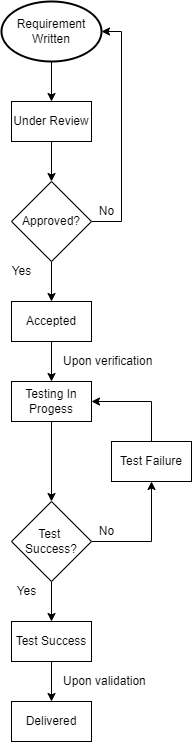
\includegraphics[height=6in]{appendices/traceability-matrix/requirement_lifecycle.png}
    \labfig{requirement_lifecycle}
\end{figure}
